\documentclass[fleqn,10pt]{wlscirep}
\title{Modeling the Coevolutionary Dynamics of the \emph{Lobaria pulmonaria} Lichen Symbiosis}

\author[1,2]{Simon Carrignon}
\author[2,3]{Salva Duran-Nebreda}
\author[2,3]{Aina Oll\'e-Vila}
\author[4]{Julia Adams}

\affil[1]{Barcelona Supercomputing Center, Carrer de Jordi Girona, 29-31, 08034 Barcelona, Spain.}
\affil[2]{Instituci\'o Catalana per a la Recerca i Estudis Avan\c{c}ats-Complex Systems Lab, Universitat Pompeu Fabra, 08003 Barcelona, Spain.}
\affil[3]{Institut de Biologia Evolutiva (CSIC-Universitat Pompeu Fabra), Passeig Mar\'itim de la Barceloneta 37, 08003 Barcelona, Spain.}
\affil[4]{Department of Botany and Plant Sciences, University of California at Riverside (UCR Lichen Herbarium), Riverside, CA 92521}


%\keywords{Keyword1, Keyword2, Keyword3}

\begin{abstract}
Example Abstract. Abstract must be under 200 words and not include subheadings or citations. Example Abstract. Abstract must be under 200 words and not include subheadings or citations. Example Abstract. Abstract must be under 200 words and not include subheadings or citations. Example Abstract. Abstract must be under 200 words and not include subheadings or citations. Example Abstract. Abstract must be under 200 words and not include subheadings or citations. Example Abstract. Abstract must be under 200 words and not include subheadings or citations. Example Abstract. Abstract must be under 200 words and not include subheadings or citations. Example Abstract. Abstract must be under 200 words and not include subheadings or citations. 
\end{abstract}
\begin{document}

\flushbottom
\maketitle
% * <john.hammersley@gmail.com> 2015-02-09T12:07:31.197Z:
%
%  Click the title above to edit the author information and abstract
%
\thispagestyle{empty}

\noindent Please note: Abbreviations should be introduced at the first mention in the main text – no abbreviations lists. Suggested structure of main text (not enforced) is provided below.

%%\section*{Introduction}

Lichens are a hyperdiverse symbiotic group spread across the globe in widely different climatic niches. The partnership between a fungus (mycobiont) and a photobiont (cyanobacteria, algae or both) allows the fungus to obtain carbohydrate-rich resources directly from their photosynthetic partner \cite{lutzoni2009lichens}. In turn, the fungus protects the photobiont from desiccation and light intensity, leading to the coevolution of the symbionts\cite{hill2009asymmetric}  and adaptive radiation into new environments \cite{nash1996lichen}. Lichenization is an evolutionarily and ecologically successful strategy ($>$20\% of fungi are lichenized), resulting in approximately 14,000 lichen species known to date \cite{lutzoni2009lichens,honegger1998lichen}. Although the nature of the lichen symbiosis is still widely debated, many sources agree that the lichen system represents an ecologically obligate mutualistic interaction whereby the net fitness of all partners is maximized~\cite{bronstein1994our,honegger1998lichen}.

%Lichens can reproduce sexually via fungal spores (horizontal transmission) and asexually via vegetative propagules and thallus fragmentation (vertical transmission). In the sexual mode of reproduction, the fungal spores must interact with a compatible free-living algae and/or cyanobacterium in order to reconstitute the lichen thallus. In the asexual mode of reproduction, mycobionts and photobionts are co-dispersed via fragmentation of the main thallus body and specialized asexual propagules.

Lichens can reproduce asexually and sexually\cite{nash1996lichen}. In the asexual mode of reproduction, mycobionts and photobionts are co-dispersed via fragmentation of the main thallus body or via specialized asexual propagules, resulting in genetically identical lichens (vertical transmission)\cite{nash1996lichen,dal2012vertical}. In the sexual mode of reproduction (horizontal transmission), the fungal spores are dispersed without the photobiont and must find a compatible algae and/or cyanobacterium in order to reconstitute the lichen thallus (\emph{relichenization}). 

The mode of reproduction strongly influences the genetic structure of lichen populations \cite{dal2012vertical,dal2011phylogeny}, affecting dispersal and evolutionary rates. 
Recently, it has been shown that {\em L. pulmonaria} mainly reproduces asexually\cite{dal2012vertical}, though sexual reproduction is suspected to play a central role at a larger evolutionary scale. The relichenization process could be a successful strategy for genetic recombination, allowing lichens to  explore wider ecological niche by sharing photobionts among different lichens, adapted to diverse local conditions. It has been hypothesized that this process could lead to the emergence of photobiont-mediated guilds, where different species of lichen interact and exchange similar photobionts within an evolutionary coherent structure\cite{rikkinen2003ecological}. These loosely integrated functional units, whereby different species can exchange resources and genetics materials, are good candidates to explain the evolutionary success of lichens. This allows different sub-components to evolve more or less independently, at different rates and under different ecological niches. This could allow the whole community to respond to environmental changes and adapt to a wider range of environmental conditions.

Studying the evolutionary dynamics of such assemblages is a difficult task because it involves a broad range of heterogeneous entities that co-evolve and interact ecologically at various spatio-temporal levels. This makes fields studies time-consuming and costly, as it requires
a lot of material from different spatio-temporal scales. Experimental work is also difficult as lichens are fragile biological entities extremely dependent on their local environmental conditions, which are complex and hard to reproduce in the laboratory\cite{nash1996lichen}.    

%This was evidenced by recent articles in the most studied lichen system: {\em L. pulmonaria}, where thalli from 62 populations in forests throughout Europe, North America, Asia, and Africa were genotyped at several hypervariable microsatellite loci \cite{dal2012vertical}. These studies concluded that the {\em L. pulmonaria-S. reticulata} symbiosis showed significant within-population genetic structure due to restricted gene flow and vertical transmission (i.e. co-dispersal of vegetative propagules). 
%
%The lichen symbiosis is extremely interesting, as the nature of the system is different from the widely studied plant-animal mutualistic systems \cite{rohr2014structural,bascompte2006asymmetric,bascompte2006structure,bastolla2009architecture,rezende2007non,guimaraes2011evolution}. Its different modes of reproduction, the fact that you find events of delichenization throughout evolution  \cite{lutzoni2001major} and that non of the partners is mobile (only throughout spores), make of it a rather particular system. Moreover, it has been conjectured the asymetry in the coevolution of the two species, due to a limited capacity of adaptation in the photobiont \cite{hill2009asymmetric} as well as that the relationship between the two species cannot always be considered a mutualism but rather a comensalism or even parasitism (with the fungi taking advantage over the photobiont)  \cite{ahmadjian1993lichen}. 

One solution to overcome these obstacles is to use of computer simulations, which allows the study of a wide range of parameters involving a massive number of heterogeneous entities. 
In order to unveil the potential factors driving the evolution of the lichen symbiosis and broader ecological and evolutionary interactions, we constructed an agent-based model based on the widely used ECHO framework \cite{holland1999echoing,holland1995hidden}. The ECHO model typically consists of a collection of entities living in a simplified spatial domain, which can move around and interact with one another and with their environment. The interactions among agents can be used to model different kinds of processes -such as mating-, and are driven by locality as well as agent-specific properties, namely the agents' genotypes. The ECHO model is also a continuous genetic algorithm \cite{mitchell1998introduction}; upon reproduction old genotypes are copied with slight mutations, giving rise to quantifiable evolutionary dynamics.

In our case, we used the tag system of ECHO to model the molecular recognition (receptors and physical embedding) between algae and fungi necessary to create the lichen. We considered two different lichenization functions based on similarity, sigmoid (hill function with $n=2$) and Michaelis-Menten (saturation dynamics). Additionally, other ecologically relevant features such as dispersal rates (introduced here as random walks) and the ratio between sexual and asexual reproduction were included in the model. Simulations were carried out assuming a wide range of ecological relationships between the algae and fungi: competition (both algae and fungi are better off on their own), parasitism (only one type of agent benefits from the partnership) and mutualism (both agents benefit).

To legitimatize the choice and the design of our model, we crossed the study of the simulations' results with empirical evidences. We first show the ability of our model to reproduce simple dynamics already well studied and understood. Then, we demonstrate that this ability can be scaled up through a 'bottom-up' approach to different levels of increasing complexity before generalising to encompass all levels of interaction, from simple well-known biological processes to broad interspecies co-evolutionary dynamics.

At the empirical level, we first used a dataset from \cite{dal2012vertical} to understand the very local processes of dispersion and reproduction of the {\em L. pulmonaria} lichen.
Using tools from network theory, we show that our model can successfully reproduce dynamics and general properties exhibited by populations, implying that the implemented processes are consistent with the biological ones. In a second approach, we studied a dataset from \cite{dal2014molecular}. In this case, some key features of the interactions between different lichen species are measured from wider populations. We used our model to show that those key features can indeed emerge from the generalization and the expansion of the same process previously described if particular conditions are met. 

Given the ability of our model to reproduce the first level of dynamics, we hope to push our simulations further to see if the emergence of more complex entities is possible, and if it is the case, under which conditions. We expect our results to support the validity of the photobiont-mediated guilds hypothesis. This would unveil important factors driving the evolutionary dynamics of the lichen symbiosis, and through that, shed new light on how species co-evolve in complex ecological communities.

\section*{Acknowledgements}
This work was initiated at the 2016 Complex Systems Summer School (CSSS) at the Sante Fe Institute (SFI). The authors would like to thank all SFI resident faculty members, SFI external faculty members, SFI Omidyar Postdoctoral Fellows, and 2016 CSSS course participants for productive discussions as well as SFI staff during the 2016 CSSS. The authors would also like to thank Dr. Christoph Scheidegger for access to multiple datasets and Dr. Francesco Dal Grande for providing detailed knowledge of the \emph{L. pulmonaria} system. 

\bibliography{../source/bib/simon}

%%The Introduction section, of referenced text\cite{Figueredo:2009dg} expands on the background of the work (some overlap with the Abstract is acceptable). The introduction should not include subheadings.
%%
%%\section*{Results}
%%
%%Up to three levels of \textbf{subheading} are permitted. Subheadings should not be numbered.
%%
%%\subsection*{Subsection}
%%
%%Example text under a subsection. Bulleted lists may be used where appropriate, e.g.
%%
%%\begin{itemize}
%%\item First item
%%\item Second item
%%\end{itemize}
%%
%%\subsubsection*{Third-level section}
%% 
%%Topical subheadings are allowed.
%%
%%\section*{Discussion}
%%
%%The Discussion should be succinct and must not contain subheadings.
%%
%%\section*{Methods}
%%
%%Topical subheadings are allowed. Authors must ensure that their Methods section includes adequate experimental and characterization data necessary for others in the field to reproduce their work.
%%
%%\bibliography{sample}
%%
%%\noindent LaTeX formats citations and references automatically using the bibliography records in your .bib file, which you can edit via the project menu. Use the cite command for an inline citation, e.g.  \cite{Figueredo:2009dg}.
%%
%%\section*{Acknowledgements (not compulsory)}
%%
%%Acknowledgements should be brief, and should not include thanks to anonymous referees and editors, or effusive comments. Grant or contribution numbers may be acknowledged.
%%
%%\section*{Author contributions statement}
%%
%%Must include all authors, identified by initials, for example:
%%A.A. conceived the experiment(s),  A.A. and B.A. conducted the experiment(s), C.A. and D.A. analysed the results.  All authors reviewed the manuscript. 
%%
%%\section*{Additional information}
%%
%%To include, in this order: \textbf{Accession codes} (where applicable); \textbf{Competing financial interests} (mandatory statement). 
%%
%%The corresponding author is responsible for submitting a \href{http://www.nature.com/srep/policies/index.html#competing}{competing financial interests statement} on behalf of all authors of the paper. This statement must be included in the submitted article file.
%%
%%\begin{figure}[ht]
%%\centering
%%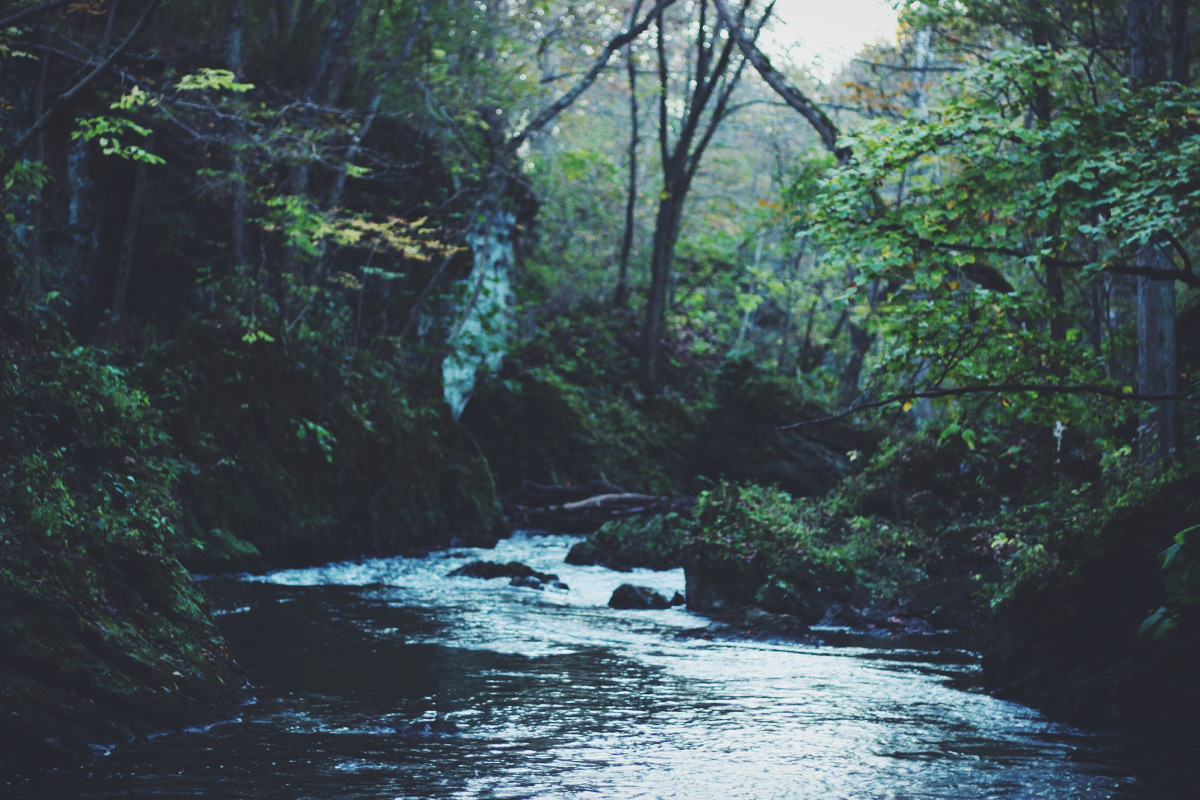
\includegraphics[width=\linewidth]{stream}
%%\caption{Legend (350 words max). Example legend text.}
%%\label{fig:stream}
%%\end{figure}
%%
%%\begin{table}[ht]
%%\centering
%%\begin{tabular}{|l|l|l|}
%%\hline
%%Condition & n & p \\
%%\hline
%%A & 5 & 0.1 \\
%%\hline
%%B & 10 & 0.01 \\
%%\hline
%%\end{tabular}
%%\caption{\label{tab:example}Legend (350 words max). Example legend text.}
%%\end{table}
%%
%%Figures and tables can be referenced in LaTeX using the ref command, e.g. Figure \ref{fig:stream} and Table \ref{tab:example}.
%%
\end{document}
